% Options for packages loaded elsewhere
\PassOptionsToPackage{unicode}{hyperref}
\PassOptionsToPackage{hyphens}{url}
\PassOptionsToPackage{dvipsnames,svgnames,x11names}{xcolor}
%
\documentclass[
  number,
  preprint,
  3p]{elsarticle}

\usepackage{amsmath,amssymb}
\usepackage{iftex}
\ifPDFTeX
  \usepackage[T1]{fontenc}
  \usepackage[utf8]{inputenc}
  \usepackage{textcomp} % provide euro and other symbols
\else % if luatex or xetex
  \usepackage{unicode-math}
  \defaultfontfeatures{Scale=MatchLowercase}
  \defaultfontfeatures[\rmfamily]{Ligatures=TeX,Scale=1}
\fi
\usepackage{lmodern}
\ifPDFTeX\else  
    % xetex/luatex font selection
\fi
% Use upquote if available, for straight quotes in verbatim environments
\IfFileExists{upquote.sty}{\usepackage{upquote}}{}
\IfFileExists{microtype.sty}{% use microtype if available
  \usepackage[]{microtype}
  \UseMicrotypeSet[protrusion]{basicmath} % disable protrusion for tt fonts
}{}
\makeatletter
\@ifundefined{KOMAClassName}{% if non-KOMA class
  \IfFileExists{parskip.sty}{%
    \usepackage{parskip}
  }{% else
    \setlength{\parindent}{0pt}
    \setlength{\parskip}{6pt plus 2pt minus 1pt}}
}{% if KOMA class
  \KOMAoptions{parskip=half}}
\makeatother
\usepackage{xcolor}
\setlength{\emergencystretch}{3em} % prevent overfull lines
\setcounter{secnumdepth}{5}
% Make \paragraph and \subparagraph free-standing
\ifx\paragraph\undefined\else
  \let\oldparagraph\paragraph
  \renewcommand{\paragraph}[1]{\oldparagraph{#1}\mbox{}}
\fi
\ifx\subparagraph\undefined\else
  \let\oldsubparagraph\subparagraph
  \renewcommand{\subparagraph}[1]{\oldsubparagraph{#1}\mbox{}}
\fi


\providecommand{\tightlist}{%
  \setlength{\itemsep}{0pt}\setlength{\parskip}{0pt}}\usepackage{longtable,booktabs,array}
\usepackage{calc} % for calculating minipage widths
% Correct order of tables after \paragraph or \subparagraph
\usepackage{etoolbox}
\makeatletter
\patchcmd\longtable{\par}{\if@noskipsec\mbox{}\fi\par}{}{}
\makeatother
% Allow footnotes in longtable head/foot
\IfFileExists{footnotehyper.sty}{\usepackage{footnotehyper}}{\usepackage{footnote}}
\makesavenoteenv{longtable}
\usepackage{graphicx}
\makeatletter
\def\maxwidth{\ifdim\Gin@nat@width>\linewidth\linewidth\else\Gin@nat@width\fi}
\def\maxheight{\ifdim\Gin@nat@height>\textheight\textheight\else\Gin@nat@height\fi}
\makeatother
% Scale images if necessary, so that they will not overflow the page
% margins by default, and it is still possible to overwrite the defaults
% using explicit options in \includegraphics[width, height, ...]{}
\setkeys{Gin}{width=\maxwidth,height=\maxheight,keepaspectratio}
% Set default figure placement to htbp
\makeatletter
\def\fps@figure{htbp}
\makeatother

\usepackage{algorithm}
\usepackage{algpseudocode}
\makeatletter
\@ifpackageloaded{tcolorbox}{}{\usepackage[skins,breakable]{tcolorbox}}
\@ifpackageloaded{fontawesome5}{}{\usepackage{fontawesome5}}
\definecolor{quarto-callout-color}{HTML}{909090}
\definecolor{quarto-callout-note-color}{HTML}{0758E5}
\definecolor{quarto-callout-important-color}{HTML}{CC1914}
\definecolor{quarto-callout-warning-color}{HTML}{EB9113}
\definecolor{quarto-callout-tip-color}{HTML}{00A047}
\definecolor{quarto-callout-caution-color}{HTML}{FC5300}
\definecolor{quarto-callout-color-frame}{HTML}{acacac}
\definecolor{quarto-callout-note-color-frame}{HTML}{4582ec}
\definecolor{quarto-callout-important-color-frame}{HTML}{d9534f}
\definecolor{quarto-callout-warning-color-frame}{HTML}{f0ad4e}
\definecolor{quarto-callout-tip-color-frame}{HTML}{02b875}
\definecolor{quarto-callout-caution-color-frame}{HTML}{fd7e14}
\makeatother
\makeatletter
\makeatother
\makeatletter
\makeatother
\makeatletter
\@ifpackageloaded{caption}{}{\usepackage{caption}}
\AtBeginDocument{%
\ifdefined\contentsname
  \renewcommand*\contentsname{Table of contents}
\else
  \newcommand\contentsname{Table of contents}
\fi
\ifdefined\listfigurename
  \renewcommand*\listfigurename{List of Figures}
\else
  \newcommand\listfigurename{List of Figures}
\fi
\ifdefined\listtablename
  \renewcommand*\listtablename{List of Tables}
\else
  \newcommand\listtablename{List of Tables}
\fi
\ifdefined\figurename
  \renewcommand*\figurename{Figure}
\else
  \newcommand\figurename{Figure}
\fi
\ifdefined\tablename
  \renewcommand*\tablename{Table}
\else
  \newcommand\tablename{Table}
\fi
}
\@ifpackageloaded{float}{}{\usepackage{float}}
\floatstyle{ruled}
\@ifundefined{c@chapter}{\newfloat{codelisting}{h}{lop}}{\newfloat{codelisting}{h}{lop}[chapter]}
\floatname{codelisting}{Listing}
\newcommand*\listoflistings{\listof{codelisting}{List of Listings}}
\makeatother
\makeatletter
\@ifpackageloaded{caption}{}{\usepackage{caption}}
\@ifpackageloaded{subcaption}{}{\usepackage{subcaption}}
\makeatother
\makeatletter
\@ifpackageloaded{tcolorbox}{}{\usepackage[skins,breakable]{tcolorbox}}
\makeatother
\makeatletter
\@ifundefined{shadecolor}{\definecolor{shadecolor}{rgb}{.97, .97, .97}}
\makeatother
\makeatletter
\makeatother
\makeatletter
\makeatother
\journal{Journal of Multivariate Analysis}
\ifLuaTeX
  \usepackage{selnolig}  % disable illegal ligatures
\fi
\usepackage[]{natbib}
\bibliographystyle{elsarticle-num-names}
\IfFileExists{bookmark.sty}{\usepackage{bookmark}}{\usepackage{hyperref}}
\IfFileExists{xurl.sty}{\usepackage{xurl}}{} % add URL line breaks if available
\urlstyle{same} % disable monospaced font for URLs
\hypersetup{
  pdftitle={Studying the Performance of the Jellyfish Optimiser for the Application of Projection Pursuit},
  pdfauthor={Alice Anonymous; Bob Security; Cat Memes; Derek Zoolander},
  pdfkeywords={projection pursuit, optimization, jellyfish
optimiser, data visualisation, high-dimensional data},
  colorlinks=true,
  linkcolor={blue},
  filecolor={Maroon},
  citecolor={Blue},
  urlcolor={Blue},
  pdfcreator={LaTeX via pandoc}}

\setlength{\parindent}{6pt}
\begin{document}

\begin{frontmatter}
\title{Studying the Performance of the Jellyfish Optimiser for the
Application of Projection Pursuit}
\author[1]{Alice Anonymous%
\corref{cor1}%
}
 \ead{alice@example.com} 
\author[2]{Bob Security%
%
}
 \ead{bob@example.com} 
\author[2]{Cat Memes%
%
}
 \ead{cat@example.com} 
\author[]{Derek Zoolander%
%
}
 \ead{derek@example.com} 

\affiliation[1]{organization={Some Institute of Technology, Department
Name},addressline={Street Address},city={City},postcode={Postal
Code},postcodesep={}}
\affiliation[2]{organization={Another University, Department
Name},addressline={Street Address},city={City},postcode={Postal
Code},postcodesep={}}

\cortext[cor1]{Corresponding author}




        
\begin{abstract}
This is the abstract. Lorem ipsum dolor sit amet, consectetur adipiscing
elit. Vestibulum augue turpis, dictum non malesuada a, volutpat eget
velit. Nam placerat turpis purus, eu tristique ex tincidunt et. Mauris
sed augue eget turpis ultrices tincidunt. Sed et mi in leo porta
egestas. Aliquam non laoreet velit. Nunc quis ex vitae eros aliquet
auctor nec ac libero. Duis laoreet sapien eu mi luctus, in bibendum leo
molestie. Sed hendrerit diam diam, ac dapibus nisl volutpat vitae.
Aliquam bibendum varius libero, eu efficitur justo rutrum at. Sed at
tempus elit.
\end{abstract}





\begin{keyword}
    projection pursuit \sep optimization \sep jellyfish
optimiser \sep data visualisation \sep 
    high-dimensional data
\end{keyword}
\end{frontmatter}
    \ifdefined\Shaded\renewenvironment{Shaded}{\begin{tcolorbox}[frame hidden, borderline west={3pt}{0pt}{shadecolor}, sharp corners, boxrule=0pt, interior hidden, enhanced, breakable]}{\end{tcolorbox}}\fi

\emph{Let's use British English (``American or British usage is
accepted, but not a mixture of these'')}

\begin{verbatim}
Warning: package 'ggplot2' was built under R version 4.3.2
\end{verbatim}

\begin{verbatim}
Warning: package 'tidyr' was built under R version 4.3.2
\end{verbatim}

\hypertarget{introduction-nicolas-and-jessica}{%
\section{Introduction {[}Nicolas and
Jessica{]}}\label{introduction-nicolas-and-jessica}}

The artificial jellyfish search (JS) algorithm \citep{chou_novel_2021}
is a swarm-based metaheuristic optimisation algorithm inspired by the
search behaviour of jellyfish in the ocean. It is one of the newest
swarm intelligence algorithms \citep{rajwar_exhaustive_2023}, which was
shown to have stronger search ability and faster convergence with few
algorithmic parameters compared to classic optimization methods
\citep{chou_novel_2021}-\citep{chou_recent_2022}.

Effective optimisation is an important aspect of many methods employed
for visualising high-dimensional data (\(X\)). Here we are concerned
about computing informative linear projections of high-dimensional
(\(p\)) data using projection pursuit (PP) (\citet{kr69}, \citet{FT74}).
This involves optimising a function (e.g. \citet{hall1989polynomial},
\citet{cook1993projection}, \citet{lee2010projection},
\citet{Loperfido2018}, \citet{Loperfido2020}), called the projection
pursuit index (PPI), that defines what is interesting or informative in
a projection.

These PPI are defined on projections (\(XA\)), which means that there is
a constraint that needs to be considered when optimising. A projection
of data is defined by a \(p\times d\) orthonormal matrix \(A\), and this
imposes the constraint on the elements of \(A\), that columns need have
norm equal to 1 and the product of columns need to sum to zero.

\citet{cook1995grand} introduced the PP guided tour, which enabled
interactive visualisation of the optimisation in order to visually
explore high-dimensional data. It is implemented in the R \citep{R}
package \texttt{tourr} \citep{tourr}. The optimisation that is
implemented is fairly basic, and potential problems were highlighted by
\citet{RJ-2021-105}. Implementing better optimisation functionality is a
goal, but it needs to be kept in mind that the guided tour also has
places importance on watching the projected data as the optimisation
progresses.

Here we explore the potential for a jellyfish optimisation to be
integrated with the guided tour. Section~\ref{sec-background} explains
the optimisation that is used in the current the projection pursuit
guided tour. Section~\ref{sec-theory} provides more details on the
jellyfish optimiser and formalises several characteristics of projection
pursuit indexes that are help to measure optimisaer performance.
Section~\ref{sec-simulation} describes a simulation study on performance
of the jellyfish for several types of data and index functions.
Section~\ref{sec-conclusion} summarises the work and provides
suggestions for future directions.

\hypertarget{sec-background}{%
\section{Projection pursuit, index functions and optimisation {[}Di and
Sherry{]}}\label{sec-background}}

A tour on high-dimensional data is constructed by geodesically
interpolating between pairs of planes. Any plane is described by an
orthonormal basis, \(A_t\), where \(t\) represents time in the sequence.
The term ``geodesic'' refers to maintaining the orthonormality
constraint so that each view shown is correctly a projection of the
data. The PP guided tour operates by geodesically interpolating to
target planes (projections) which have high PP index values, as provided
by the optimiser. The geodesic interpolation means that the viewer sees
a continuous sequence of projections of the data, so they can watch
patterns of interest forming as the function is optimised. There are
five optimisation methods implemented in the \texttt{tourr} package:

\begin{itemize}
\tightlist
\item
  \texttt{search\_geodesic()}: provides a pseudo-derivative
  optimisation. It searches locally for the best direction, based on
  differencing the index values for very close projections. Then it
  follows the direction along the geodesic path between planes, stopping
  when the next index value fails to increase.
\item
  \texttt{search\_better()}: is a brute-force optimisation searching
  randomly for projections with higher index values.
\item
  \texttt{search\_better\_random()}: is essentially simulated annealing
  \citep{Bertsimas93} where the search space is reduced as the
  optimisation progresses.
\item
  \texttt{search\_posse()}: implements the algorithm described in
  \citet{posse95}.
\item
  \texttt{search\_polish()}: is a very localised search, to take tiny
  steps to get closer to the local maximum.
\end{itemize}

There are several PP index functions available: \texttt{holes()} and
\texttt{cmass()} \citep{cook1993projection}; \texttt{lda\_pp()}
\citep{lee2005projection}; \texttt{pda\_pp()} \citep{lee2010projection};
\texttt{dcor2d()} and \texttt{splines2d()} \citep{Grimm2016};
\texttt{norm\_bin()} and \texttt{norm\_kol()} \citep{huber85};
\texttt{slice\_index()} \citep{Laa:2020wkm}. Most are relatively simply
defined, for any projection dimension, and implemented because they are
relatively easy to optimise. A goal is to be able to incorporate more
complex PP indexes, for example based on scagnostics (\citet{scag},
\citet{WW08}).

An initial investigation of PP indexes, and the potential for
scagnostics is described in \citet{laa_using_2020}. To be useful here an
optimiser needs to be able to handle functions which are not very
smooth. In addition, because data structures might be relatively fine,
the optimiser needs to be able to find maxima that occur with a small
squint angle, that can only be seen from very close by. One last aspect
that is useful is for an optimiser to return local maxima in addition to
global because data can contain many different and interesting features.

\hypertarget{sec-theory}{%
\section{The jellyfish optimiser and properties of PP indexes {[}Nicolas
and Jessica{]}}\label{sec-theory}}

The jellyfish optimiser (JSO) mimics the natural movements of jellyfish,
which include passive and active motions driven by ocean currents and
their swimming patterns, respectively. In the context of optimization,
these movements are abstracted to explore the search space in a way that
balances exploration (searching new areas) and exploitation (focusing on
promising areas). The algorithm aims to find the optimal solution by
adapting the jellyfish's behaviour to navigate towards the best solution
over iterations \citep{chou_novel_2021}.

To understand what the jellyfish optimizer is doing in the context of
Projection Pursuit, we first start with a current projection (the
starting point). Then, we evaluate this projection using an index
function, which tells us how good the current projection is. We then
move the projection in a direction determined by the `best jelly' and
random factors, influenced by how far along we are in the optimization
process (the trial \(i\) and \texttt{max.tries}). Occasionally, we might
explore completely new directions like a jellyfish might with ocean
currents. Then, we compare new potential projections to our current one.
If they're better, we adopt them; if not, we stick with our current
projection. This process continues and iteratively improves the
projection, until we reach the maximum number of trials.

\begin{tcolorbox}[enhanced jigsaw, title={Algorithm: Jellyfish Optimizer Pseudo Code}, bottomrule=.15mm, colframe=quarto-callout-note-color-frame, bottomtitle=1mm, titlerule=0mm, toprule=.15mm, colback=white, colbacktitle=quarto-callout-note-color!10!white, opacityback=0, opacitybacktitle=0.6, leftrule=.75mm, toptitle=1mm, coltitle=black, breakable, arc=.35mm, left=2mm, rightrule=.15mm]

\textbf{Input}: \texttt{current\_projections}, \texttt{index\_function},
\texttt{tries}, \texttt{max\_tries}

\textbf{Output}: \texttt{optimized\_projection}

\textbf{Initialize} \texttt{best\_jelly} as the projection with the best
index value from \texttt{current\_projections}, and
\texttt{current\_index} as the array of index values for each projection
in \texttt{current\_projections}

\textbf{for} each try in 1 to max\_tries \textbf{do}

\begin{quote}
Calculate \(c_t\) based on the current try and max\_tries
\end{quote}

\begin{quote}
\textbf{if} \(c_t\) is greater than or equal to \(0.5\) \textbf{then}

\begin{quote}
Define trend based on the best jelly and current projections
\end{quote}

\begin{quote}
Update each projection towards the trend using a random factor and
orthonormalisation
\end{quote}

\textbf{else}

\begin{quote}
\textbf{if} a random number is greater than \(1 - c_t\) \textbf{then}

\begin{quote}
Slightly adjust each projection with a small random factor (Type A
passive)
\end{quote}

\textbf{else}

\begin{quote}
For each projection, compare with a random jelly and adjust towards or
away from it (Type B active)
\end{quote}
\end{quote}

Update the orientation of each projection to maintain consistency

Evaluate the new projections using the index function
\end{quote}

\begin{quote}
\textbf{if} any new projection is worse than the current, revert to the
\texttt{current\_projection} for that case

\begin{quote}
Determine the projection with the best index value as the new
best\_jelly
\end{quote}
\end{quote}

\begin{quote}
\textbf{if} the try is the last one, print the final best projection and
\textbf{exit}
\end{quote}

\textbf{return} the set of projections with the updated best\_jelly as
the optimized\_projection

\end{tcolorbox}

The JSO implementation involves several key parameters that control its
search process in optimization problems. These parameters are designed
to guide the exploration and exploitation phases of the algorithm. While
the specific implementation details can vary depending on the version of
the algorithm or its application, we focus on two main parameters that
are most relevant to our application: the number of jellyfish and drift.

\citet{laa_using_2020} has proposed five criteria for assessing
projection pursuit indexes (smoothness, squintability, flexibility,
rotation invariance, and speed). Since not all the properties affects
the execution of the optimisation, here we consider the three relevant
properties (smoothness, squintability, and speed), and propose three
metrics to evaluate these three properties.

\hypertarget{smoothness}{%
\subsection{Smoothness}\label{smoothness}}

If we evaluate the index function at some random points (like the random
initialization of the jellyfish optimizer), then we can interpret these
random index values as a random field, indexed by a space parameter: the
random projection angle. This analogy suggests to use this random
training sample to fit a spatial model, a simple one being a (spatial)
Gaussian process.

How can we define a measure of smoothness from this? The distribution of
a Gaussian process is fully determined by its mean function and
covariance function. The way the covariance function is defined is where
smoothness comes into play: if an index is very smooth, then two close
projection angles should produce close index values (strong
correlation); by contrast, if an index is not smooth, then two close
projection angles might give very different index values (fast decay of
correlations with respect to distance between angles).

Popular covariance functions are parametric positive semi-definite
functions, some of which have a parameter to capture the smoothness of
the Gaussian field. In particular, consider the Matérn class of
covariance functions, defined by

\[
K(u):=\frac{(\sqrt{2\nu}u)^{\nu}}{\Gamma(\nu)2^{\nu-1}}\mathcal{K}_{\nu}(\sqrt{2\nu}u)
\]

where \(\nu>0\) is the smoothness parameter and where
\(\mathcal{K}_\nu\) is the modified Bessel function. The Matérn
covariance function can be expressed analytically when \(\nu\) is a
half-integer, the most popular values in the literature being \(1/2\),
\(3/2\) and \(5/2\) . The parameter \(\nu\), called smoothness
parameter, controls the decay of the covariance function. As such, it is
an appropriate measure of smoothness of a random field.

In our context, we suggest to use this parameter as a measure of the
smoothness of the index function by fitting a Gaussian process prior
with Matérn covariance on a dataset generated by random evaluations of
the index function, as in the initial stage of the jellyfish random
search. There exist several R packages, such as GpGp or ExaGeoStatR, to
fit the hyperparameters of a GP covariance function on data. In this
project, we make use of the GpGp package.

The fitted value \(\nu>0\) can be interpreted as follows: the higher
\(\nu\), the smoother the index function.

\hypertarget{squintability}{%
\subsection{Squintability}\label{squintability}}

From the literature, it is commonly understood that a large squint angle
implies that the function is easy to optimize, because we do not need to
be very close to the perfect view to see the structure. A small squint
angle means that the derivative of the index function can still be very
large values near the optimal point and will rapidly change as we get
even closer to the optimum. As such we can observe the second order
gradient, which is the rate of change of gradient, over the space we are
searching. For some index functions, the second order gradient is not
well-defined, we can approximate the second order gradient vector in
similar fashion as the above section.

To the best of our knowledge, this is the first attempt to measure the
notion of squintability.

\hypertarget{speed}{%
\subsection{Speed}\label{speed}}

The speed of optimizing an index function can be calculated/measured
using the computational complexity (in big O notation, with respect to
the sample size) of computing the index function.

\hypertarget{sec-simulation}{%
\section{Application {[}Di and Sherry{]}}\label{sec-simulation}}

The jellyfish optimiser has been implemented in the tourr package
\citep{wickham_tourr_2011} and we will use the diagnostic plots proposed
in the ferrn package \citep{RJ-2021-105} to visualise the optimisation
process.

\hypertarget{going-beyond-10d}{%
\subsection{Going beyond 10D}\label{going-beyond-10d}}

The pipe-finding problem is initially used to investigate indexes and
optimisers in \citet{laa_using_2020}, and we extend it from a 6D problem
to a 12D problem.

Jellyfish optimiser, as a multi-start algorithm, is efficient in
{[}\ldots{]} for high-dimensional problems

\begin{figure}

{\centering 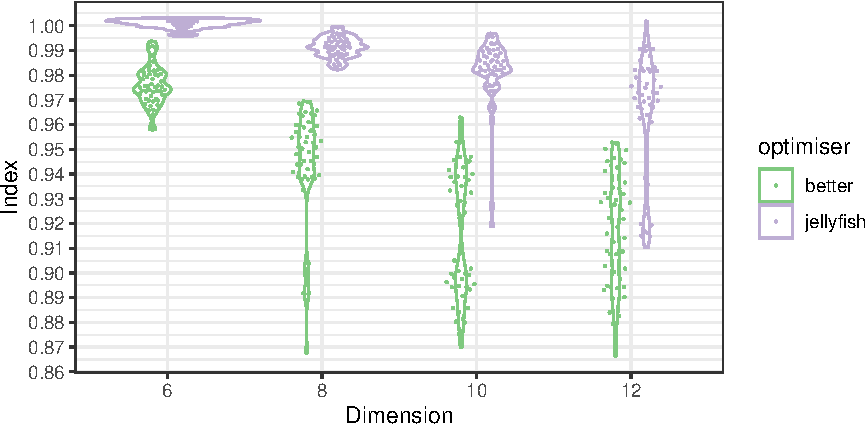
\includegraphics{optim_files/figure-pdf/unnamed-chunk-2-1.pdf}

}

\caption{sthis sdfaksdlf}

\end{figure}

\begin{figure}

{\centering 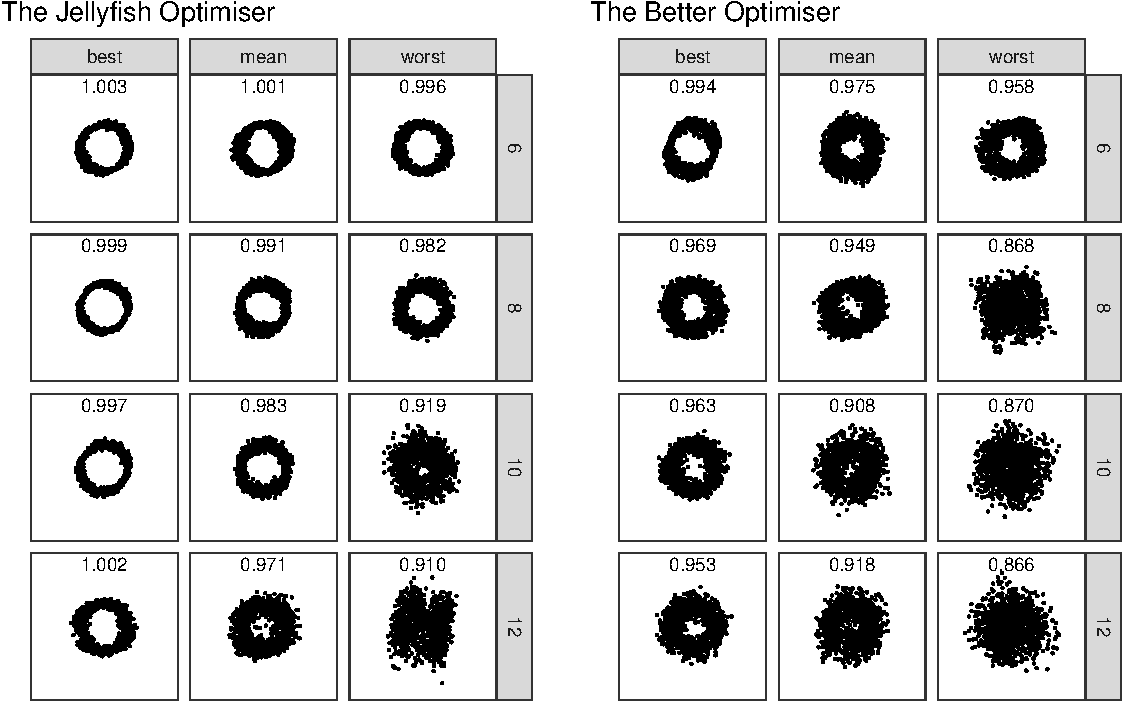
\includegraphics{optim_files/figure-pdf/unnamed-chunk-3-1.pdf}

}

\caption{sthis sdfaksdlf}

\end{figure}

\hypertarget{on-skewness-and-kurtosis-index}{%
\subsection{On skewness and kurtosis
index}\label{on-skewness-and-kurtosis-index}}

\hypertarget{another-data-example}{%
\subsection{Another data example}\label{another-data-example}}

\hypertarget{sec-conclusion}{%
\section{Conclusion {[}Di and Sherry{]}}\label{sec-conclusion}}


\renewcommand\refname{References}
  \bibliography{bibliography.bib}


\end{document}
